\documentclass[]{article}
\usepackage{lmodern}
\usepackage{amssymb,amsmath}
\usepackage{ifxetex,ifluatex}
\usepackage{fixltx2e} % provides \textsubscript
\ifnum 0\ifxetex 1\fi\ifluatex 1\fi=0 % if pdftex
  \usepackage[T1]{fontenc}
  \usepackage[utf8]{inputenc}
\else % if luatex or xelatex
  \ifxetex
    \usepackage{mathspec}
  \else
    \usepackage{fontspec}
  \fi
  \defaultfontfeatures{Ligatures=TeX,Scale=MatchLowercase}
\fi
% use upquote if available, for straight quotes in verbatim environments
\IfFileExists{upquote.sty}{\usepackage{upquote}}{}
% use microtype if available
\IfFileExists{microtype.sty}{%
\usepackage{microtype}
\UseMicrotypeSet[protrusion]{basicmath} % disable protrusion for tt fonts
}{}
\usepackage[margin=1in]{geometry}
\usepackage{hyperref}
\hypersetup{unicode=true,
            pdftitle={Problem Set 1},
            pdfauthor={Elmer Camargo},
            pdfborder={0 0 0},
            breaklinks=true}
\urlstyle{same}  % don't use monospace font for urls
\usepackage{color}
\usepackage{fancyvrb}
\newcommand{\VerbBar}{|}
\newcommand{\VERB}{\Verb[commandchars=\\\{\}]}
\DefineVerbatimEnvironment{Highlighting}{Verbatim}{commandchars=\\\{\}}
% Add ',fontsize=\small' for more characters per line
\usepackage{framed}
\definecolor{shadecolor}{RGB}{248,248,248}
\newenvironment{Shaded}{\begin{snugshade}}{\end{snugshade}}
\newcommand{\AlertTok}[1]{\textcolor[rgb]{0.94,0.16,0.16}{#1}}
\newcommand{\AnnotationTok}[1]{\textcolor[rgb]{0.56,0.35,0.01}{\textbf{\textit{#1}}}}
\newcommand{\AttributeTok}[1]{\textcolor[rgb]{0.77,0.63,0.00}{#1}}
\newcommand{\BaseNTok}[1]{\textcolor[rgb]{0.00,0.00,0.81}{#1}}
\newcommand{\BuiltInTok}[1]{#1}
\newcommand{\CharTok}[1]{\textcolor[rgb]{0.31,0.60,0.02}{#1}}
\newcommand{\CommentTok}[1]{\textcolor[rgb]{0.56,0.35,0.01}{\textit{#1}}}
\newcommand{\CommentVarTok}[1]{\textcolor[rgb]{0.56,0.35,0.01}{\textbf{\textit{#1}}}}
\newcommand{\ConstantTok}[1]{\textcolor[rgb]{0.00,0.00,0.00}{#1}}
\newcommand{\ControlFlowTok}[1]{\textcolor[rgb]{0.13,0.29,0.53}{\textbf{#1}}}
\newcommand{\DataTypeTok}[1]{\textcolor[rgb]{0.13,0.29,0.53}{#1}}
\newcommand{\DecValTok}[1]{\textcolor[rgb]{0.00,0.00,0.81}{#1}}
\newcommand{\DocumentationTok}[1]{\textcolor[rgb]{0.56,0.35,0.01}{\textbf{\textit{#1}}}}
\newcommand{\ErrorTok}[1]{\textcolor[rgb]{0.64,0.00,0.00}{\textbf{#1}}}
\newcommand{\ExtensionTok}[1]{#1}
\newcommand{\FloatTok}[1]{\textcolor[rgb]{0.00,0.00,0.81}{#1}}
\newcommand{\FunctionTok}[1]{\textcolor[rgb]{0.00,0.00,0.00}{#1}}
\newcommand{\ImportTok}[1]{#1}
\newcommand{\InformationTok}[1]{\textcolor[rgb]{0.56,0.35,0.01}{\textbf{\textit{#1}}}}
\newcommand{\KeywordTok}[1]{\textcolor[rgb]{0.13,0.29,0.53}{\textbf{#1}}}
\newcommand{\NormalTok}[1]{#1}
\newcommand{\OperatorTok}[1]{\textcolor[rgb]{0.81,0.36,0.00}{\textbf{#1}}}
\newcommand{\OtherTok}[1]{\textcolor[rgb]{0.56,0.35,0.01}{#1}}
\newcommand{\PreprocessorTok}[1]{\textcolor[rgb]{0.56,0.35,0.01}{\textit{#1}}}
\newcommand{\RegionMarkerTok}[1]{#1}
\newcommand{\SpecialCharTok}[1]{\textcolor[rgb]{0.00,0.00,0.00}{#1}}
\newcommand{\SpecialStringTok}[1]{\textcolor[rgb]{0.31,0.60,0.02}{#1}}
\newcommand{\StringTok}[1]{\textcolor[rgb]{0.31,0.60,0.02}{#1}}
\newcommand{\VariableTok}[1]{\textcolor[rgb]{0.00,0.00,0.00}{#1}}
\newcommand{\VerbatimStringTok}[1]{\textcolor[rgb]{0.31,0.60,0.02}{#1}}
\newcommand{\WarningTok}[1]{\textcolor[rgb]{0.56,0.35,0.01}{\textbf{\textit{#1}}}}
\usepackage{graphicx,grffile}
\makeatletter
\def\maxwidth{\ifdim\Gin@nat@width>\linewidth\linewidth\else\Gin@nat@width\fi}
\def\maxheight{\ifdim\Gin@nat@height>\textheight\textheight\else\Gin@nat@height\fi}
\makeatother
% Scale images if necessary, so that they will not overflow the page
% margins by default, and it is still possible to overwrite the defaults
% using explicit options in \includegraphics[width, height, ...]{}
\setkeys{Gin}{width=\maxwidth,height=\maxheight,keepaspectratio}
\IfFileExists{parskip.sty}{%
\usepackage{parskip}
}{% else
\setlength{\parindent}{0pt}
\setlength{\parskip}{6pt plus 2pt minus 1pt}
}
\setlength{\emergencystretch}{3em}  % prevent overfull lines
\providecommand{\tightlist}{%
  \setlength{\itemsep}{0pt}\setlength{\parskip}{0pt}}
\setcounter{secnumdepth}{0}
% Redefines (sub)paragraphs to behave more like sections
\ifx\paragraph\undefined\else
\let\oldparagraph\paragraph
\renewcommand{\paragraph}[1]{\oldparagraph{#1}\mbox{}}
\fi
\ifx\subparagraph\undefined\else
\let\oldsubparagraph\subparagraph
\renewcommand{\subparagraph}[1]{\oldsubparagraph{#1}\mbox{}}
\fi

%%% Use protect on footnotes to avoid problems with footnotes in titles
\let\rmarkdownfootnote\footnote%
\def\footnote{\protect\rmarkdownfootnote}

%%% Change title format to be more compact
\usepackage{titling}

% Create subtitle command for use in maketitle
\providecommand{\subtitle}[1]{
  \posttitle{
    \begin{center}\large#1\end{center}
    }
}

\setlength{\droptitle}{-2em}

  \title{Problem Set 1}
    \pretitle{\vspace{\droptitle}\centering\huge}
  \posttitle{\par}
  \subtitle{MGSC 310, Fall 2019, Professor Hersh}
  \author{Elmer Camargo}
    \preauthor{\centering\large\emph}
  \postauthor{\par}
    \date{}
    \predate{}\postdate{}
  

\begin{document}
\maketitle

\begin{Shaded}
\begin{Highlighting}[]
\KeywordTok{library}\NormalTok{(ISLR)}
\KeywordTok{data}\NormalTok{(Auto)}
\KeywordTok{plot}\NormalTok{(cars)}
\end{Highlighting}
\end{Shaded}

\begin{center}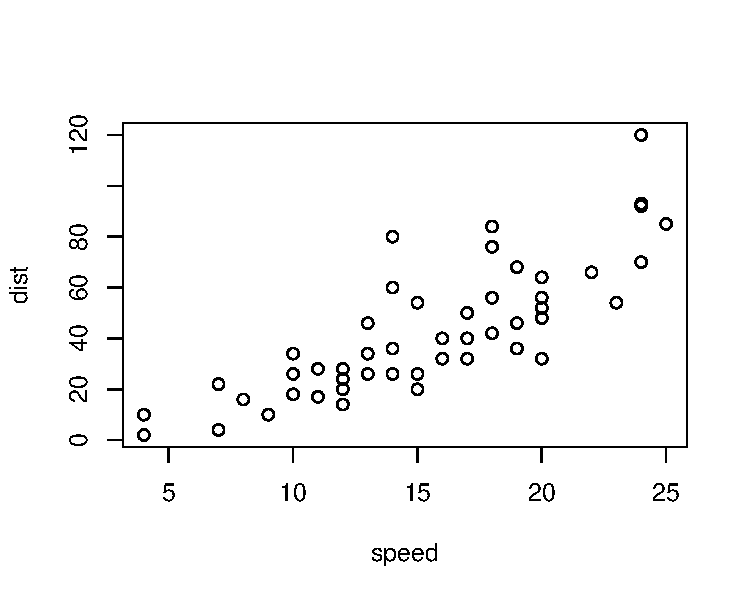
\includegraphics{RMarkdown_Pset_Template_files/figure-latex/unnamed-chunk-1-1} \end{center}

\hypertarget{question-1-these-are-headings-note-the}{%
\subsection{Question 1 (These are headings, note the
`\#')}\label{question-1-these-are-headings-note-the}}

This is text. I can write text just like this and it will come out as a
paragraph.

If I want to do a bulleted list

\begin{itemize}
\tightlist
\item
  I
\item
  can
\item
  do
\item
  one
\item
  quite
\item
  easily

  \begin{itemize}
  \tightlist
  \item
    sub-bullets are cool too
  \end{itemize}
\end{itemize}

\begin{enumerate}
\def\labelenumi{\arabic{enumi}.}
\item
  Numbered lists are easy too
\item
  Just add numbers!

  \begin{enumerate}
  \def\labelenumii{\alph{enumii})}
  \tightlist
  \item
    letters are cool too.
  \end{enumerate}
\end{enumerate}

\hypertarget{an-introduction-to-code-snippets.}{%
\subsection{2. An introduction to code
snippets.}\label{an-introduction-to-code-snippets.}}

Adding code to your document is done using these code ``chunks''. Code
chunks look like the code below, they start with
``\texttt{"\ and\ end\ with\ "}''. After the first `````'' you must
specify the code language to use (in this case ``r''). The code will be
executed and outputted when you output your document.

You can have rich text in your documents such as \emph{italics} by
encasing the italicised word in one "*``. \textbf{Bold} works the same
but has two''**"s.

\begin{Shaded}
\begin{Highlighting}[]
\KeywordTok{setwd}\NormalTok{(}\StringTok{'C:/Users/Elmer/Documents/R/Statistical Modeling/PSET1'}\NormalTok{)}
\KeywordTok{library}\NormalTok{(ISLR)}
\KeywordTok{data}\NormalTok{(Auto)}
\KeywordTok{plot}\NormalTok{(cars)}
\end{Highlighting}
\end{Shaded}

\begin{center}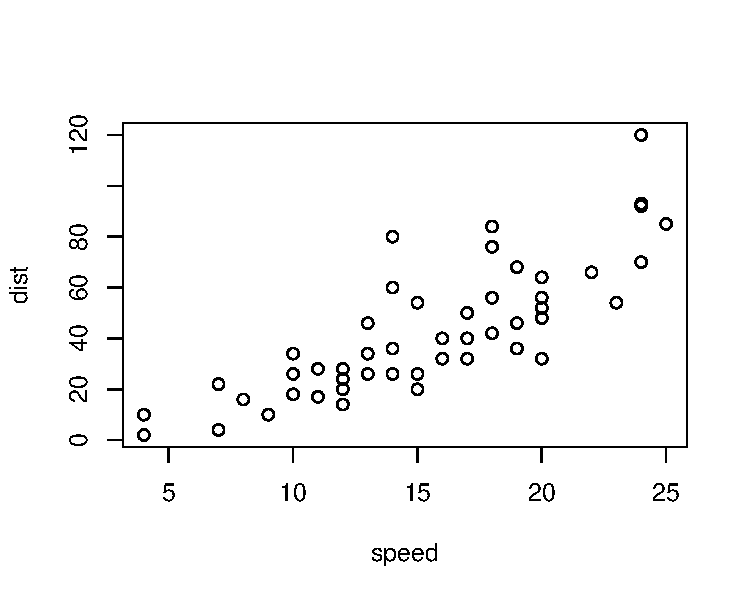
\includegraphics{RMarkdown_Pset_Template_files/figure-latex/unnamed-chunk-2-1} \end{center}

\hypertarget{question-3}{%
\subsection{Question 3}\label{question-3}}

You can put in any type of code in your code chunk. You can execute
lines of code by highlighting your cursor in the code chunk and
executing it line by line using CTRL + RETURN (or COMMAND + RETURN on
Macs) as you would in the editor.

\begin{Shaded}
\begin{Highlighting}[]
\KeywordTok{names}\NormalTok{(Auto)}
\CommentTok{## [1] "mpg"          "cylinders"    "displacement" "horsepower"  }
\CommentTok{## [5] "weight"       "acceleration" "year"         "origin"      }
\CommentTok{## [9] "name"}
\NormalTok{mod1 <-}\StringTok{ }\KeywordTok{lm}\NormalTok{(mpg }\OperatorTok{~}\StringTok{ }\NormalTok{weight }\OperatorTok{+}\StringTok{ }\NormalTok{year }\OperatorTok{+}\StringTok{ }\NormalTok{horsepower, }\DataTypeTok{data =}\NormalTok{ Auto)}
\KeywordTok{summary}\NormalTok{(mod1)}
\CommentTok{## }
\CommentTok{## Call:}
\CommentTok{## lm(formula = mpg ~ weight + year + horsepower, data = Auto)}
\CommentTok{## }
\CommentTok{## Residuals:}
\CommentTok{##     Min      1Q  Median      3Q     Max }
\CommentTok{## -8.7911 -2.3220 -0.1753  2.0595 14.3527 }
\CommentTok{## }
\CommentTok{## Coefficients:}
\CommentTok{##               Estimate Std. Error t value Pr(>|t|)    }
\CommentTok{## (Intercept) -1.372e+01  4.182e+00  -3.281  0.00113 ** }
\CommentTok{## weight      -6.448e-03  4.089e-04 -15.768  < 2e-16 ***}
\CommentTok{## year         7.487e-01  5.212e-02  14.365  < 2e-16 ***}
\CommentTok{## horsepower  -5.000e-03  9.439e-03  -0.530  0.59663    }
\CommentTok{## ---}
\CommentTok{## Signif. codes:  0 '***' 0.001 '**' 0.01 '*' 0.05 '.' 0.1 ' ' 1}
\CommentTok{## }
\CommentTok{## Residual standard error: 3.43 on 388 degrees of freedom}
\CommentTok{## Multiple R-squared:  0.8083, Adjusted R-squared:  0.8068 }
\CommentTok{## F-statistic: 545.4 on 3 and 388 DF,  p-value: < 2.2e-16}
\end{Highlighting}
\end{Shaded}

\hypertarget{question-4}{%
\subsection{Question 4}\label{question-4}}

When you are done with your RMarkdown file, you can create an output
file by clicking the button ``Knit'' above. You have three output
options, HTML, PDF, and Word. Word output is fine. If you want to
produce PDF files you need to first
\href{https://miktex.org/download}{install Miktex} a popular Latex
framework. (Latex is a mathematical programming language.)

\begin{figure}
\centering
\includegraphics{images/rmarkdown.png}
\caption{Oh yea, this is how you include images. This is the image
caption}
\end{figure}

\hypertarget{advanced-stuff}{%
\subsection{Advanced stuff}\label{advanced-stuff}}

Some more tutorials are recommended if you really want to produce cool
documents:

\begin{itemize}
\tightlist
\item
  {[}\url{https://rmarkdown.rstudio.com/authoring_basics.html}{]}(\url{https://rmarkdown.rstudio.com/authoring_basics.html}
\item
  \url{https://ourcodingclub.github.io/2016/11/24/rmarkdown-1.html}
\item
  \url{https://rmarkdown.rstudio.com/lesson-1.html}
\item
  \url{https://www.rstudio.com/wp-content/uploads/2015/02/rmarkdown-cheatsheet.pdf}
\end{itemize}

You can do \(latex\) math by using ``\$'' as in
\(Y = X\beta + \epsilon\)


\end{document}
